\section{Результаты симуляций}

В одном из запусков тестового измерения, описанного в главе\,\ref{sec:timeTestsGSI}, источник отсутствовал. Поэтому, записанные сигналы порождались космическими лучами, случайными фотонами, проникшими через стенки чёрного ящика, и шумовыми одноэлектронными сигналами. Уровень триггера, определяющий условие записи сигнала был установлен достаточно низко, чтобы одноэлектронные шумовые сигналы преодолели этот порог. С помощью анализа форм одноэлектронных шумовых сигналов был определен параметр $b$ функции\,\ref{eq:1electronSIM}, характеризующий форму одноэлектронного сигнала при моделировании сигналов в \er.

На Рис.\ref{ris:1pesignalexp} изображён один из шумовых сигналов, профитированный функцией\,\ref{eq:1electronSIM}. 

{
	\centering
	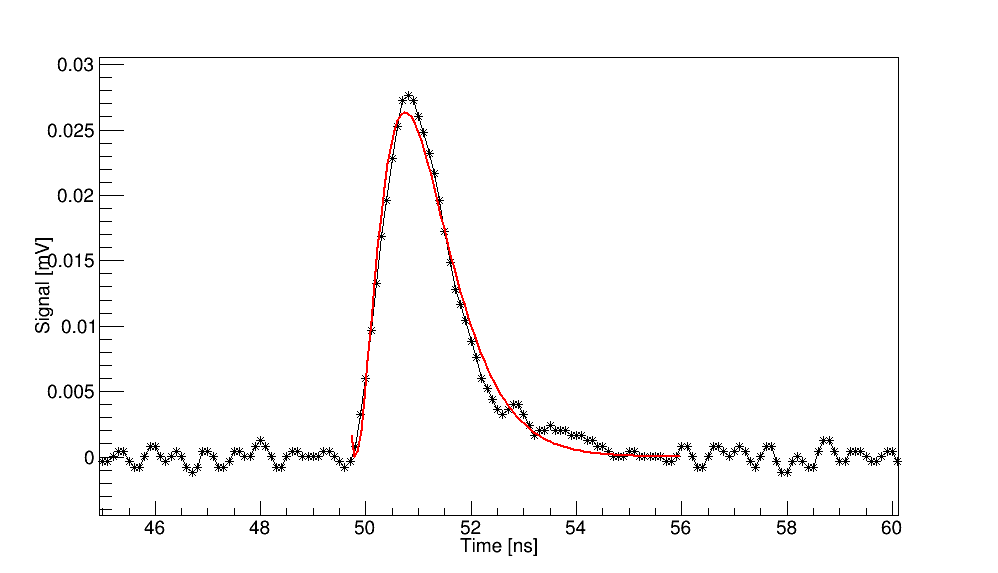
\includegraphics[width=\linewidth]{1pesignalexp.png}
	\captionof{figure}{Анализ формы одноэлектронного шумового сигнала}\label{ris:1pesignalexp}
}

Были обработаны десятки таких сигналов, из которых было рассчитано среднее $\bar{b}=0.45$, которое использовалось в моделировании эксперимента в \er.

В результате моделирования эксперимента с прототипом NeuRad в \er\, были получены формы сигналов, визуально похожие на те, которые мы видели в эксперименте, см. Рис.\ref{ris:compare}.

\begin{figure}[!ht]
	\centering
	\begin{tabular}{cc}
		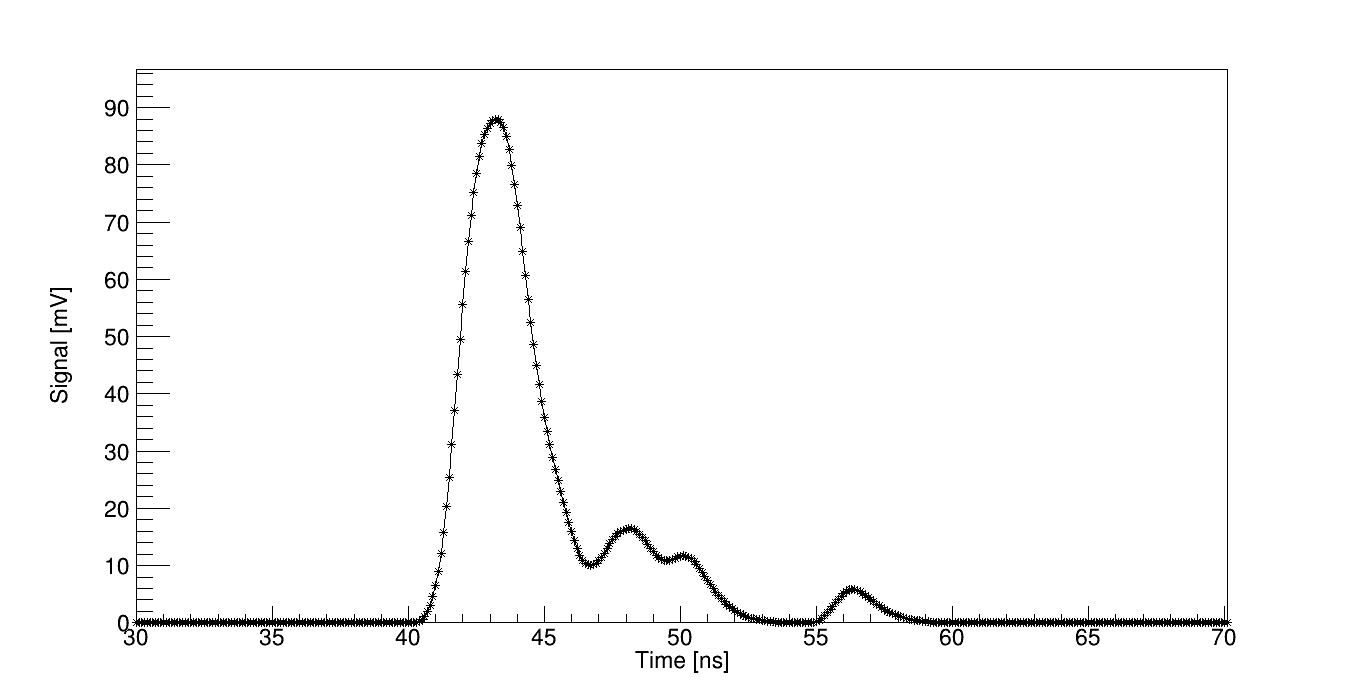
\includegraphics[width=0.52\linewidth]{simSignal1.png} 
		&
		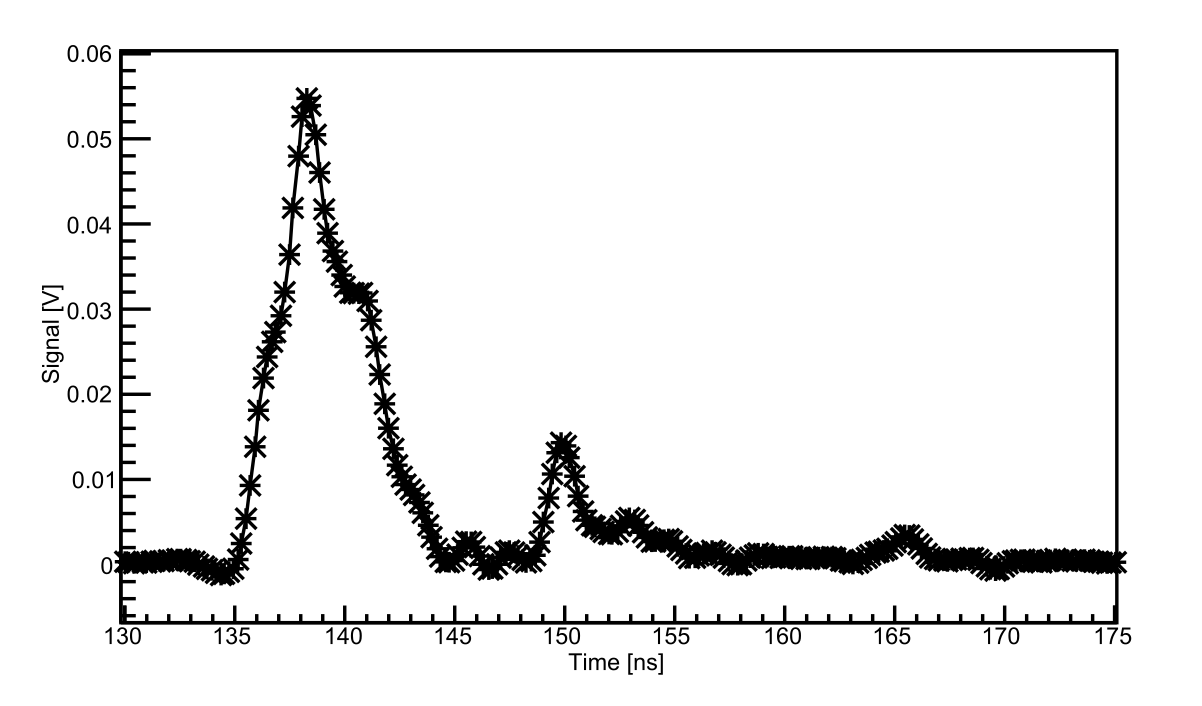
\includegraphics[width=0.48\linewidth]{originalsignalform.png} \\
		а) & б)
	\end{tabular}
	%		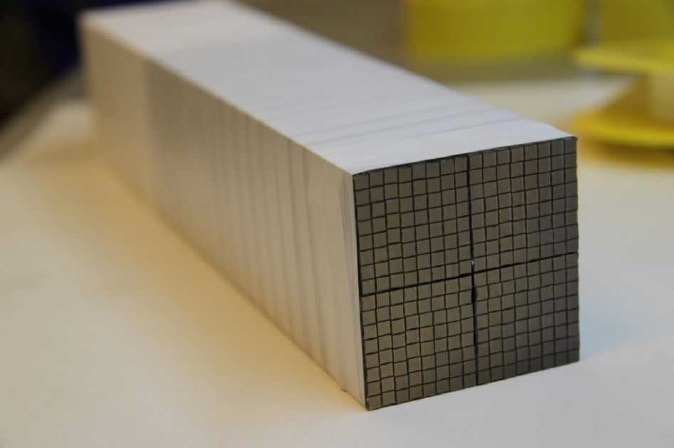
\includegraphics[width=0.5\linewidth]{neuradfibers.png}
	\caption[Short caption for list of figures]{а) Типичный сигнал записанный фреймворком \er\ при симуляции эксперимента с прототипом  NeuRad. б) Типичный сигнал записанный осциллографом в эксперименте.}
	\label{ris:compare}
\end{figure}

С помощью суммарной формы сигнала, Рис.\ref{ris:integralSim}, был оценено время высвечивания сцинтиллятора: 6\,нс. 

{
	\centering
	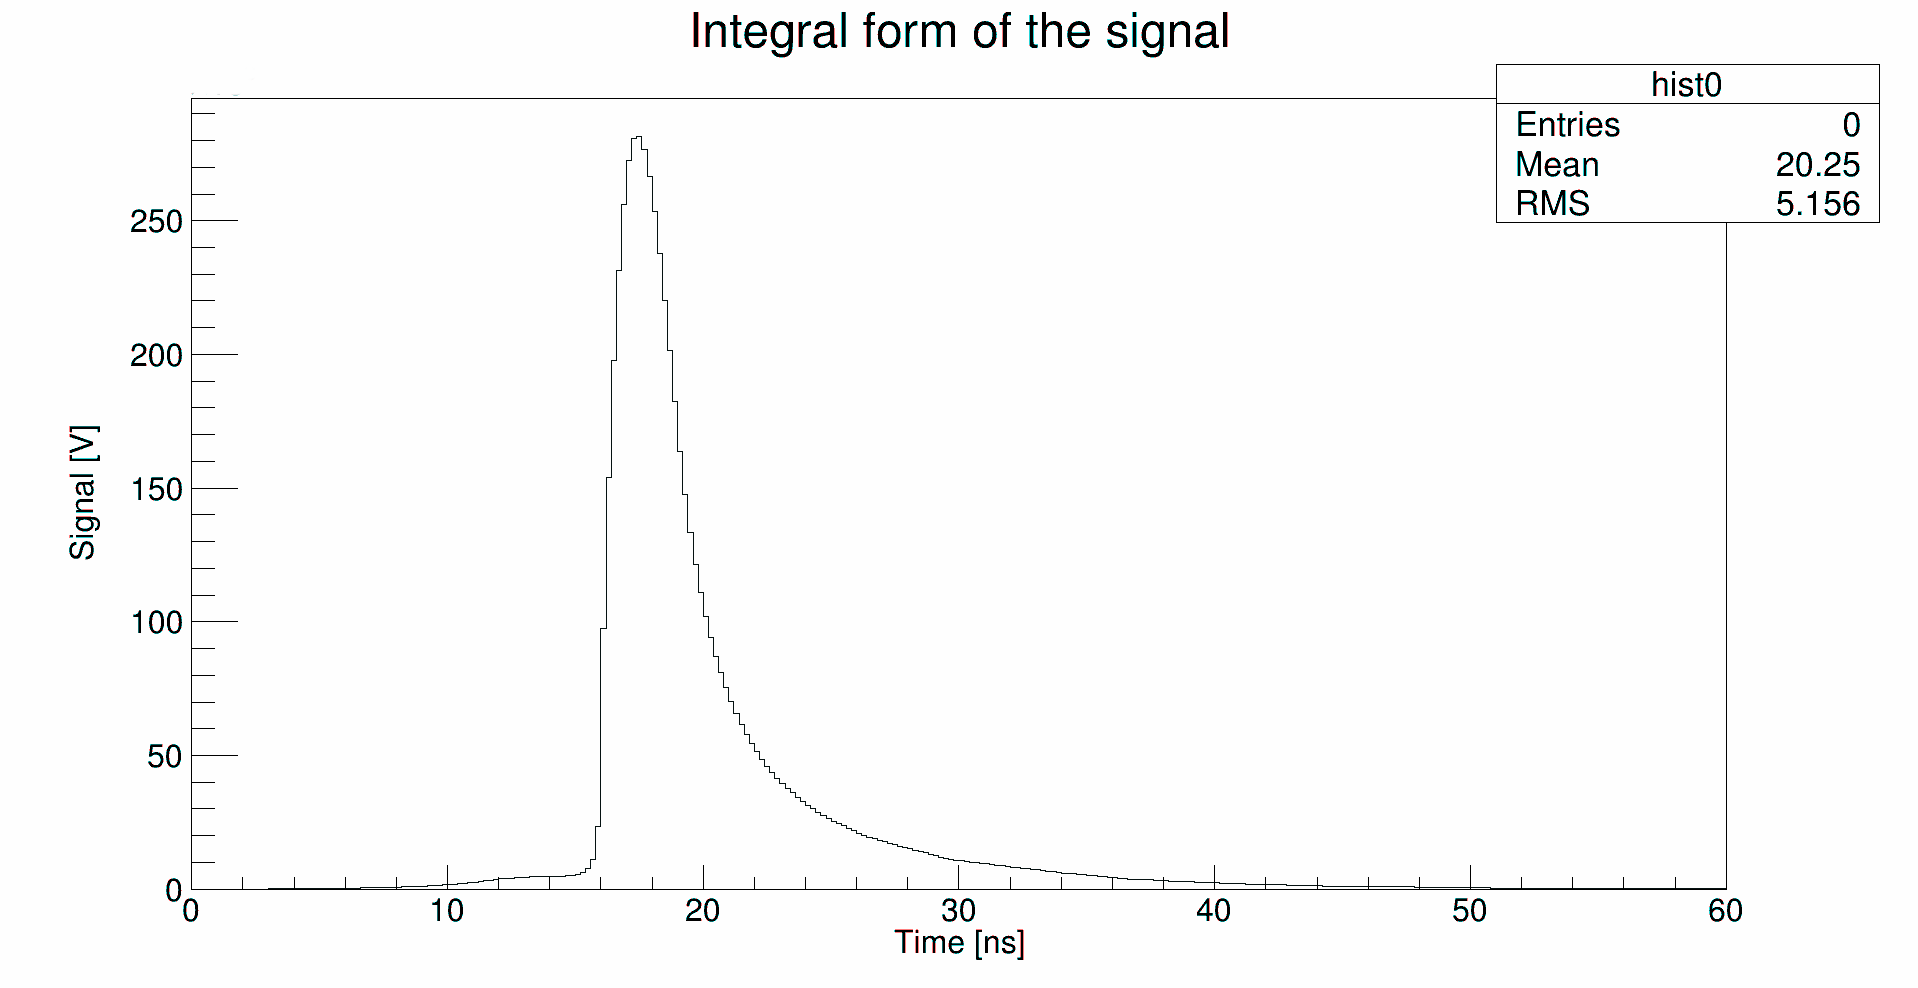
\includegraphics[width=\linewidth]{integralSim.png}
	\captionof{figure}{Суммарная форма сигналов анода в \er}\label{ris:integralSim}
}

К полученным в результате моделирования эксперимента сигналам были применены такие же алгоритмы обработки, внедрённые в \er. 

Результаты обработки данных с виртуального эксперимента были схожи с результатами обработки экспериментальных данных. На Рис.\ref{ris:tausim} показано сравнение распределений $\Delta\tau$ полученных из экспериментальных и моделированных данных. Времена сигналов в данном случае рассчитывались методом анализа переднего фронта сигнала и равнялись временем превышения передним фронтом сигнала значения, равного половине амплитуды первого локального максимума.

{
	\centering
	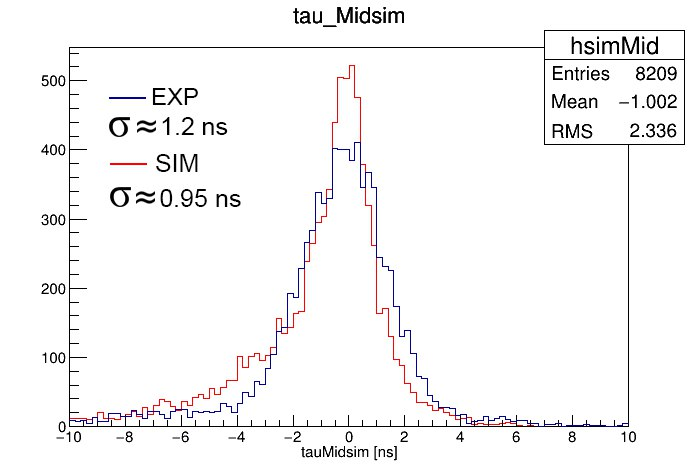
\includegraphics[width=\linewidth]{tausim.png}
	\captionof{figure}{Распределение $\Delta\tau$ рассчитанное методом анализа переднего фронта для экспериментальных (синим цветом) и моделированных (красным) данных}\label{ris:tausim}
}
	
На Рис.\ref{ris:ampsim} изображено сравнение амплитудно-временных корреляций для моделированных, справа, и экспериментальных, слева, данных. 

{
	\centering
	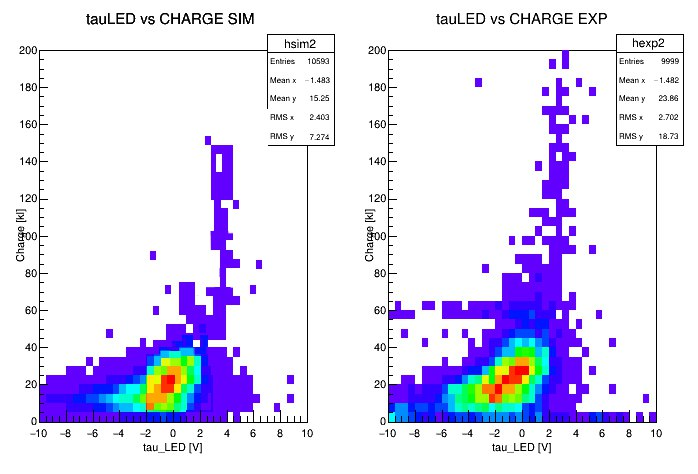
\includegraphics[width=\linewidth]{ampsim.png}
	\captionof{figure}{Зависимость $\Delta\tau$ рассчитанное методом дискриминатора переднего фронта от заряда. Слева для моделированных, справа для экспериментальных данных }\label{ris:ampsim}
}

%Результаты расчётов временного разрешения прототипа NeuRad с помощью симуляции в \er/ записаны в таблице\,\ref{tab:simresults}.
%
%{
%	\centering
%	\begin{tabular}{|c|c|c|}
%		\hline
%		\textbf{Метод}: & Параметры & $\sigma$/FWHM[нс]\\
%		\hline
%		CFD: & Задержка  1,5\,нс, коэффициент ослабления 0,3 & 0,5/1,18\\
%		\hline
%		LED: & Порог 20\,мВ &  0,42/1\\
%		\hline
%		Анализ фронта 50\%: & Порог 20\,мВ &  0,8/1,88\\
%		\hline
%		Анализ фронта 10\%: & Порог 20\,мВ &  0,52/1,23\\
%		\hline
%	\end{tabular}
%	\captionof{table}{ Результаты рассчётов временного разрешения прототипа NeuRad в \er.}\label{tab:simresults}
%}

